\section{Introduzione}
L'\acrfull{adrr} è la base dati centralizzata utilizzata da EUROCONTROL \citep{eurocontrol2025} per gestire in maniera integrata le informazioni sullo spazio aereo europeo lungo l’intero ciclo di pianificazione e di controllo del traffico aereo.  
L’ADR supporta il programma \gls{dmean}, iniziativa che mira a ottimizzare l’utilizzo dello spazio aereo coordinando in tempo quasi reale le decisioni di \gls{asm} e di \gls{atfcm}.

Accanto alla versione operativa, \citet{eurocontrol2025} pubblica \acrfull{adrr}: un sottoinsieme storico anonimizzato del repository, destinato alla comunità scientifica e reso scaricabile tramite il portale OneSky Online \cite{eurocontrol2025onesky}.

\section{Domini informativi}
Nel contesto dell’\gls{adr} un dominio informativo è una partizione logica del modello dati che raggruppa, secondo criteri tematici e funzionali, insiemi omogenei di entità e relativi attributi.  
Ogni dominio descrive un particolare aspetto del sistema \gls{atm} ad esempio aerodromi, rotte o regolazioni \gls{atfcm} e contiene esclusivamente oggetti tra loro coerenti sotto il profilo semantico. Tale organizzazione permette di ottenere:
\begin{description}
  \item[Modularità] Consente di suddividere la base dati in unità gestibili, semplificando la manutenzione, il controllo delle versioni e l’attribuzione delle responsabilità.
  
  \item[Governance] Collega a ciascun dominio un proprietario del dato, specifiche regole di qualità e procedure di validazione dedicate, assicurando la tracciabilità.

  \item[Efficienza delle interrogazioni] Permette alle applicazioni di recuperare soltanto i sotto-insiemi informativi pertinenti al caso d’uso, riducendo latenza e carico computazionale.

  \item[Allineamento operativo] Mantiene coerenza fra il modello logico dei dati e i processi operativi (\gls{asm} e \gls{atfcm}), agevolando l’integrazione con i flussi di lavoro reali.
\end{description}

\citet{eurocontrol2025adr} individua undici domini logici (Tabella.~\ref{tab:domini}), ciascuno modellato secondo lo schema \acrshort{aixm}\,5.1. I domini variano da informazioni statiche a entità che possono cambiare più volte al giorno.

\begin{table}[htbp]
  \centering
  \begin{tabular}{ll}
    \toprule
    \textbf{Dominio} & \textbf{Esempi di oggetti/attributi}\\
    \midrule
    Aerodrome & Indicatore \acrshort{icao}, \acrshort{arp}, configurazioni pista\\
    Aircraft Type & Codici \acrshort{icao}/\acrshort{iata}\\
    Airspace & \gls{fir}, settori, aree \acrshort{fua}\\
    \gls{atfcm} Scenario & Regolazioni, configurazioni di rete\\
    Authority & Ente normativo o gestore\\
    Capacity & Volumi di traffico, regolazioni\\
    Route & \acrshort{ats}, \acrshort{cdr}, rotte oceaniche \acrshort{nat}\\
    Significant Point & \acrshort{navaid}, punti \acrshort{rnav}\\
    Terminal Procedures & \acrshort{sid}, \acrshort{star}, avvicinamenti\\
    Flight Restrictions & \acrshort{rad}, \acrshort{dct}, \acrshort{fra}\\
    Organisational Unit & \gls{acc}, \acrshort{fmp}, \acrshort{aro}\\
    \bottomrule
  \end{tabular}
  \caption{Domini informativi principali del repository \gls{adr}.}
  \label{tab:domini}
\end{table}
\section{Ciclo di vita dei dati}
L'\gls{adr} segue il ciclo \gls{airac}, un sistema standardizzato che garantisce aggiornamenti coordinati e tempestivi delle informazioni aeronautiche ogni 28 giorni, assicurando coerenza e sincronizzazione tra tutti gli attori coinvolti nel sistema \gls{atm}.

Le principali fasi temporali che scandiscono il ciclo \gls{airac} sono descritte in dettaglio nel documento \cite{eurocontrol2025adr}, e sono qui di seguito riportate, con il supporto della Figura~\ref{fig:airac_cycle} che ne rappresenta graficamente la successione e i rapporti funzionali.
\\\\
\textbf{D} = rilascio nuovo \gls{airac} \quad
\textbf{T} = mezzanotte del cambio \acrshort{airac} \quad
\begin{description}
  \item[Design] Attività di progettazione dello spazio aereo a lungo e medio termine, comprendenti la valutazione e la definizione di procedure terminali e di rotta, svolte dalla data di entrata in vigore della precedente release fino a \textbf{D-72}.

  \item[Strategic] Inserimento e validazione dei dati statici (SDO Data Entry \& Validation), ovvero informazioni aeronautiche permanenti o di lungo periodo che non cambiano frequentemente, e pubblicazione dei dati AIRAC statici (SDO AIRAC Data Published), cioè dati pianificati in anticipo e comunicati con largo anticipo, nell'intervallo da \textbf{D-72} a \textbf{D-34}, con termine ultimo per la pubblicazione statica fissato a \textbf{D-56}.

  \item[Pre-Tactical] Raffinamento pre-tattico, pubblicazione dei dati non-AIRAC (SDO non-AIRAC Data Published), ovvero informazioni di carattere operativo che non richiedono la pianificazione anticipata prevista dal ciclo AIRAC, e rilascio degli avvisi \acrshort{notam}, avvisi urgenti e tempestivi, a partire da \textbf{D-34} fino al giorno antecedente la data di cambio AIRAC (\textbf{D-1}). La pubblicazione \acrshort{notam} può avvenire dal giorno stesso della release (\textbf{D}).

  \item[Tactical] Gestione tattica in tempo reale delle regolazioni \gls{atm}/\gls{atfcm} e delle modifiche operative, dall'ultimo giorno prima della release (\textbf{D-1}) fino al momento esatto del cambio \gls{airac} a mezzanotte (\textbf{T}).
\end{description}
\clearpage
\begin{figure}[H]
    \centering
    \begin{tikzpicture}[
    % --- Stili generali ---
    every node/.style={font=\small},
    arrowstyle/.style={-{Latex[length=3mm]}, line width=1pt},
    cyanline/.style={arrowstyle, draw=cyan!60!black},
    cyanline2/.style={draw=cyan!60!black, line width=1pt},
    greenline/.style={arrowstyle, draw=green!70!black},
    greenline2/.style={draw=green!70!black, line width=1pt},
    yellowline/.style={arrowstyle, draw=orange!25!yellow},
    yellowline2/.style={draw=orange!25!yellow, line width=1pt},
    orangeline/.style={arrowstyle, draw=orange!70!yellow},
    timeline/.style={line width=1pt},
    tick/.style={line width=1pt},
    publish/.style={fill=green!70!black, draw=none, shape=diamond, minimum size=5pt}
]

% ==========================
% 0) DEFINIZIONE COORDINATE
% ==========================
% Qui dichiariamo TUTTE le coordinate (D72, D56, D34, D28, D6, D1, T2, T0)
% PRIMA di usarle nelle righe successive.
\coordinate (D72) at (0,0);
\coordinate (D56) at (1.2,0);
\coordinate (D34) at (2.8,0);
\coordinate (D28) at (3.6,0);
\coordinate (D6) at (7,0);
\coordinate (D1) at (8,0);
\coordinate (T2) at (9,0);
\coordinate (T0) at (11,0);
\pgfmathsetmacro{\levelsep}{-0.9}

%\textbf{D} = rilascio nuovo \gls{airac} \quad
%    \textbf{T} = mezzanotte del cambio \acrshort{airac} \quad

\begin{scope}[shift={(0,1.2)}]
  \node[anchor=west,font=\small] at (-2,0) {%
    \tikz[baseline=-0.5ex] \node[diamond, draw=green!70!black, fill=green!70!black, minimum size=6pt, inner sep=0pt] {}; = inizio disponibilità  };
\end{scope}

% ==============================
% 1) LINEA PRINCIPALE E TICK
% ==============================
\draw[timeline] (-2,0) -- (T0);
\foreach \name/\lbl in {
  D72/D-72, 
  D56/D-56, 
  D34/D-34, 
  D28/D-28, 
  D6/D-6, 
  D1/D-1, 
  T2/T-2, 
  T0/T
} {
  \draw[tick] (\name) ++(0,-0.1) -- ++(0,0.2) node[above, yshift=2pt]{\lbl};
}

% ===========================================
% 2) Airspace Design Activities (freccia ciano)
% ===========================================
\coordinate (AirStart) at (-2,\levelsep); 
\coordinate (AirEnd)   at ($(D72)+(0,\levelsep)$); % primo livello
\draw[cyanline] (AirStart) -- (AirEnd)
    node[midway, above, yshift=2pt, text=cyan, align=center]{};

% ==================================================
% 3) SDO Data Entry & Validation (freccia ciano)
% ==================================================
\coordinate (SDOentryStart) at ($(D72)+(0,\levelsep*2)$);
\coordinate (SDOentryEnd)   at ($(D56)+(0,\levelsep*2)$);
\draw[cyanline] (SDOentryStart) -- (SDOentryEnd)
  node[pos=0, anchor=east, xshift=-2pt, align=center]{\acrshort{sdo} Data Entry \\\& Validation};

% =========================================================
% 4) SDO AIRAC Data Published (diamante + freccia verde fino T)
% =========================================================
\coordinate (AIRACnode) at ($ (D56) + (0,\levelsep*3) $);
\draw[greenline2] (AIRACnode) -- ($(T0) + (0,\levelsep*3)$)
  node[pos=0, anchor=east, xshift=-2pt, align=center]{\acrshort{sdo} \gls{airac}\\Data Published};
\node[diamond, draw=green!70!black, fill=green!70!black, minimum size=6pt, inner sep=0pt]
     at (AIRACnode) {};
     

% ==============================================================
% 5) SDO non-AIRAC Data Published (diamante + freccia verde fino T)
% ==============================================================
\coordinate (nonAIRACnode) at ($ (D28) + (0,\levelsep*4) $);
\draw[greenline2] (nonAIRACnode) -- ($(T0) + (0,\levelsep*4)$)
  node[pos=0, anchor=east, xshift=-2pt, align=center]{\acrshort{sdo} non-\gls{airac}\\Data Published};
\node[diamond, draw=green!70!black, fill=green!70!black, minimum size=6pt, inner sep=0pt]
     at (nonAIRACnode) {};
     
% ===========================================
% 6) NOTAM (freccia gialla da D-34 a T)
% ===========================================
\coordinate (NOTAMstart) at ($ (D56) + (0,\levelsep*5)$);
\coordinate (NOTAMend)   at ($ (T0) + (0,\levelsep*5)$);
\draw[yellowline] (NOTAMstart) -- (NOTAMend)
  node[midway, above, yshift=2pt]{\acrshort{notam}};


% =============================================================
% 7) CACD Published (diamante + freccia verde fino D-6, poi gialla)
% =============================================================
\coordinate (CACDstart) at ($ (D34) + (0,\levelsep*6)$);
\coordinate (CACDmid) at ($ (D6) + (0,\levelsep*6)$);
\coordinate (CACDend) at ($ (T0) + (0,\levelsep*6)$);

\draw[greenline2] (CACDstart) -- (CACDmid)
    node[midway, above, yshift=2pt]{\acrshort{cacd} Published}
;

\draw[yellowline2] (CACDmid) -- (CACDend)
    node[midway, above, yshift=2pt]{\acrshort{cacd} Pre-OPS}   
;

\node[diamond, draw=green!70!black, fill=green!70!black, minimum size=6pt, inner sep=0pt]
     at (CACDstart) {};


% ============================================================== 
% 8) ASM Data (freccia verde da D-72 a D-6, poi gialla fino a T)
% ============================================================== 
\coordinate (ASMstart) at ($ (D72) + (0,\levelsep*7)$);
\coordinate (ASMquarter)   at ($ (D6) + (0,\levelsep*7)$);
\coordinate (ASMmid)   at ($ (T2) + (0,\levelsep*7)$);
\coordinate (ASMend)   at ($ (T0) + (0,\levelsep*7)$);
\draw[greenline2] (ASMstart) -- (ASMquarter)
     node[midway, above, yshift=2pt]{Level 1}
     node[pos=0, anchor=east, xshift=-2pt, align=center]{\gls{asm} Data};
\draw[yellowline2] (ASMquarter) -- (ASMmid)
     node[midway, above, yshift=2pt]{Level 2};
\draw[orangeline] (ASMmid) -- (ASMend)
    node[midway, above, yshift=2pt]{Level 3};


% ===========================================================================
% 9) ATFM Data (freccia verde da D-72 a D-6, poi gialla fino a T, con etichette)
% ===========================================================================
\coordinate (ASMstart) at ($ (D72) + (0,\levelsep*8)$);
\coordinate (ASMquarter)   at ($ (D6) + (0,\levelsep*8)$);
\coordinate (ASMmid)   at ($ (T2) + (0,\levelsep*8)$);
\coordinate (ASMend)   at ($ (T0) + (0,\levelsep*8)$);
\draw[greenline2] (ASMstart) -- (ASMquarter)
     node[midway, above, yshift=2pt]{Strategic}
     node[pos=0, anchor=east, xshift=-2pt, align=center]{\gls{atfcm} Data};
\draw[yellowline2] (ASMquarter) -- (ASMmid)
     node[midway, above, yshift=2pt]{Pre-Tactical};
\draw[orangeline] (ASMmid) -- (ASMend)
    node[midway, above, yshift=2pt]{Tactical};


\coordinate (start) at (-2,\levelsep*9);
\coordinate (quarter)   at ($ (D72) + (0,\levelsep*9)$);
\coordinate (Interp) at ($ 
     (quarter) !0.2! ( $(D56)+(0,{\levelsep*9}) $ ) 
   $);
\coordinate (secondquarter)   at ($ (T2) + (0,\levelsep*9)$);
\coordinate (end)   at ($ (T0) + (0,\levelsep*9)$);

\draw[cyanline2] (start) -- (Interp)
    node[midway, above, yshift=2pt, text=black]{\textbf{Design}};

\draw[greenline2] (Interp) -- ($ (D6) + (0,\levelsep*9)$)
    node[midway, above, yshift=2pt]{\textbf{Strategic}};
;

\draw[yellowline2] ($ (D6) + (0,\levelsep*9)$) -- ($ (T2) + (0,\levelsep*9)$)
    node[midway, above, yshift=2pt]{\textbf{Pre-Tactical}};


\draw[orangeline] ($ (T2) + (0,\levelsep*9)$) -- ($ (T0) + (0,\levelsep*9)$)
    node[midway, above, yshift=2pt]{\textbf{Tactical}};


\end{tikzpicture}

    \caption{Timeline di manutenzione del ciclo \gls{airac}.}
    \label{fig:airac_cycle}
\end{figure}

\section{Copertura geografica e frequenza di aggiornamento}
La copertura geografica e la frequenza di aggiornamento dei dati differiscono significativamente a seconda del repository considerato. Di seguito è riportato un confronto tra \acrfull{adr} e \acrfull{adrr} relativamente agli aspetti principali.

\begin{table}[h!]
    \centering
    \begin{tabular}{p{3cm}p{5cm}p{5cm}}
        \toprule
         & \textbf{\acrlong{adr}} & \textbf{\acrlong{adrr}} \\[0.8em]
        \midrule
        \textbf{Copertura} & Area di competenza \acrshort{cfmu}. & Area di competenza \acrshort{cfmu}. \\[0.8em]
        \addlinespace
        \textbf{Periodo disponibile} & Tempo reale, con aggiornamenti fino a intervalli inferiori a un'ora nella fase tattica. & Dati storici dal 2015 al 2023 (circa 23,3 milioni di voli totali). \\[0.8em]
        \addlinespace
        \textbf{Selezione temporale} & Continuo, variabile secondo fase operativa (design, strategica, pre-tattica e tattica). & Mesi campione di marzo, giugno, settembre e dicembre per ciascun anno disponibile. \\[0.8em]
        \addlinespace
        \textbf{Ritardo di pubblicazione} & Immediato. & Circa due anni, per garantire anonimizzazione e tutela della privacy.
    \end{tabular}
\end{table}
\section{Struttura \gls{adrr}}
Ogni rilascio di \acrshort{adrr} consiste in un archivio compresso in formato zip, contenente tutti i file CSV pertinenti.  
Tutte le tabelle incluse negli archivi sono descritte in dettaglio nel documento~\cite{rnd2023} e sono organizzate nelle seguenti macro-aree:

\subsection{FLIGHTS}
\label{sec:flights}
\subsubsection{Tabella FLIGHTS}
La tabella FLIGHTS contiene i principali attributi di ciascun volo commerciale registrato nel sistema \gls{adrr}, inclusi orari, aeromobili e segmenti di mercato.
\begin{description}
  \item[\textbf{ECTL\_ID}] Identificativo numerico univoco del volo nel sistema \acrshort{prisme}.
  \item[\textbf{ADEP}] Codice \acrshort{icao} dell’aeroporto di partenza.
  \item[\textbf{ADEP Latitude}] Latitudine dell’aeroporto di partenza (gradi decimali).
  \item[\textbf{ADEP Longitude}] Longitudine dell’aeroporto di partenza (gradi decimali).
  \item[\textbf{ADES}] Codice \acrshort{icao} dell’aeroporto di destinazione.
  \item[\textbf{ADES Latitude}] Latitudine dell’aeroporto di destinazione (gradi decimali).
  \item[\textbf{ADES Longitude}] Longitudine dell’aeroporto di destinazione (gradi decimali).
  \item[\textbf{Filed Off Block Time}] Orario di spinta dal parcheggio pianificato (UTC).
  \item[\textbf{Filed Arrival Time}] Orario di arrivo pianificato (UTC).
  \item[\textbf{Actual Off Block Time}] Orario di spinta effettivo (UTC).
  \item[\textbf{Actual Arrival Time}] Orario di atterraggio effettivo (UTC).
  \item[\textbf{AC Type}] Designatore \acrshort{icao} del tipo di aeromobile.
  \item[\textbf{AC Operator}] Codice a tre lettere dell’operatore del volo.
  \item[\textbf{AC Registration}] Matricola dell’aeromobile.
  \item[\textbf{ICAO Flight Type}] Tipo di volo secondo \acrshort{icao} (S, N, …).
  \item[\textbf{\acrshort{statfor} Market Segment}] Segmento di mercato STATFOR.
  \item[\textbf{Requested \acrshort{fl}}] Livello di volo richiesto nel piano di volo.
  \item[\textbf{Actual Distance Flown}] Distanza percorsa (miglia nautiche).
\end{description}

\subsection{FLIGHT POINTS}
\label{sec:flight_points}
\subsubsection{Tabella FLIGHT POINTS}
La tabella FLIGHT POINTS descrive il profilo dei way‐points attraversati da ciascun volo, sia in pianificazione sia in effettivo, evidenziando tempi e livelli di volo.
\begin{description}
  \item[\textbf{ECTL\_ID}] Identificativo del volo (stesso di FLIGHTS).
  \item[\textbf{Sequence Number}] Numero sequenziale del punto attraversato.
  \item[\textbf{Time Over}] Orario di sorvolo del punto (UTC):
    \begin{itemize}
      \item \emph{filed}: tempo calcolato dal piano di volo depositato
      \item \emph{actual}: tempo derivato da osservazioni radar e \gls{atfcm}
    \end{itemize}
  \item[\textbf{Flight Level}] Livello di volo (\acrshort{fl}) al sorvolo.
  \item[\textbf{Latitude}] Latitudine del punto (gradi decimali).
  \item[\textbf{Longitude}] Longitudine del punto (gradi decimali).
\end{description}

\subsection{FLIGHT AIRSPACES}
\label{sec:flight_airspace}
\subsubsection{Tabella FLIGHT FIRs FILED}
La tabella FLIGHT FIRs FILED elenca i segmenti di spazio aereo pianificati attraversati da ciascun volo, con orari di ingresso e uscita pianificati.
\begin{description}
  \item[\textbf{ECTL\_ID}] Identificativo del volo.
  \item[\textbf{Sequence Number}] Ordine cronologico dell’attraversamento.
  \item[\textbf{FIR ID}] Identificativo della \gls{fir}.
  \item[\textbf{Entry Time}] Orario di ingresso (UTC).
  \item[\textbf{Exit Time}] Orario di uscita (UTC).
\end{description}
\textit{(Medesimi campi si applicano anche alle \acrshort{aua}, sostituendo \acrshort{aua} ID a \gls{fir} ID.)}


\subsubsection{Tabella FLIGHT FIRs ACTUAL}
La tabella FLIGHT FIRs ACTUAL riporta i medesimi segmenti di spazio aereo attraversati realmente dai voli, con orari di ingresso e uscita osservati.
\begin{description}
  \item[\textbf{ECTL\_ID}] Identificativo del volo.
  \item[\textbf{Sequence Number}] Ordine cronologico.
  \item[\textbf{FIR ID}] Identificativo dell’area attraversata.
  \item[\textbf{Entry Time}] Orario reale di ingresso (UTC).
  \item[\textbf{Exit Time}] Orario reale di uscita (UTC).
\end{description}
\textit{(Medesimi campi si applicano anche alle \acrshort{aua}, sostituendo \acrshort{aua} ID a \gls{fir} ID.)}

\subsection{\acrshort{atm} ENVIRONMENT DATA}
\label{sec:atm_env}
\subsubsection{Tabella AIRAC}
La tabella AIRAC riporta l’elenco dei cicli AIRAC validi nel periodo considerato, con relative date di inizio e fine validità.
\begin{description}
  \item[\textbf{External ID}] Identificativo del ciclo AIRAC.
  \item[\textbf{Date From}] Data di inizio validità del ciclo (UTC).
  \item[\textbf{Date To}] Data di fine validità del ciclo (UTC).
\end{description}

\subsubsection{Tabella ROUTES}
La tabella ROUTES definisce le \gls{ats} come sequenze di punti geografici ordinate da monte a valle.
\begin{description}
  \item[\textbf{Route ID}] Identificativo alfanumerico della rotta.
  \item[\textbf{Sequence Number}] Numero sequenziale del punto lungo la rotta.
  \item[\textbf{Latitude}] Latitudine del punto (gradi decimali).
  \item[\textbf{Longitude}] Longitudine del punto (gradi decimali).
\end{description}

\subsubsection{Tabella \gls{fir}}
\label{sec:table_fir}
La tabella \gls{fir} descrive il profilo dei confini delle \acrlong{fir} (o \acrshort{uir}), tramite vertici e livelli di volo estremi.
\begin{description}
  \item[\textbf{Airspace ID}] Identificativo della FIR (o UIR).
  \item[\textbf{Min Flight Level}] Livello di volo minimo del volume.
  \item[\textbf{Max Flight Level}] Livello di volo massimo del volume.
  \item[\textbf{Sequence Number}] Ordine dei vertici del poligono.
  \item[\textbf{Latitude}] Latitudine del vertice (gradi decimali).
  \item[\textbf{Longitude}] Longitudine del vertice (gradi decimali).
\end{description}
\section{Accesso e condizioni d’uso}
L’\gls{adrr} è scaricabile previa registrazione sul portale OneSky Online~\cite{eurocontrol2025onesky}.  
La procedura richiede i seguenti passaggi illustrati in Figura~\ref{fig:accesso_conditions}.

\begin{figure}[H]
  \centering
  % --- prima coppia di immagini ---
  \begin{subfigure}[b]{0.5\textwidth}
    \centering
    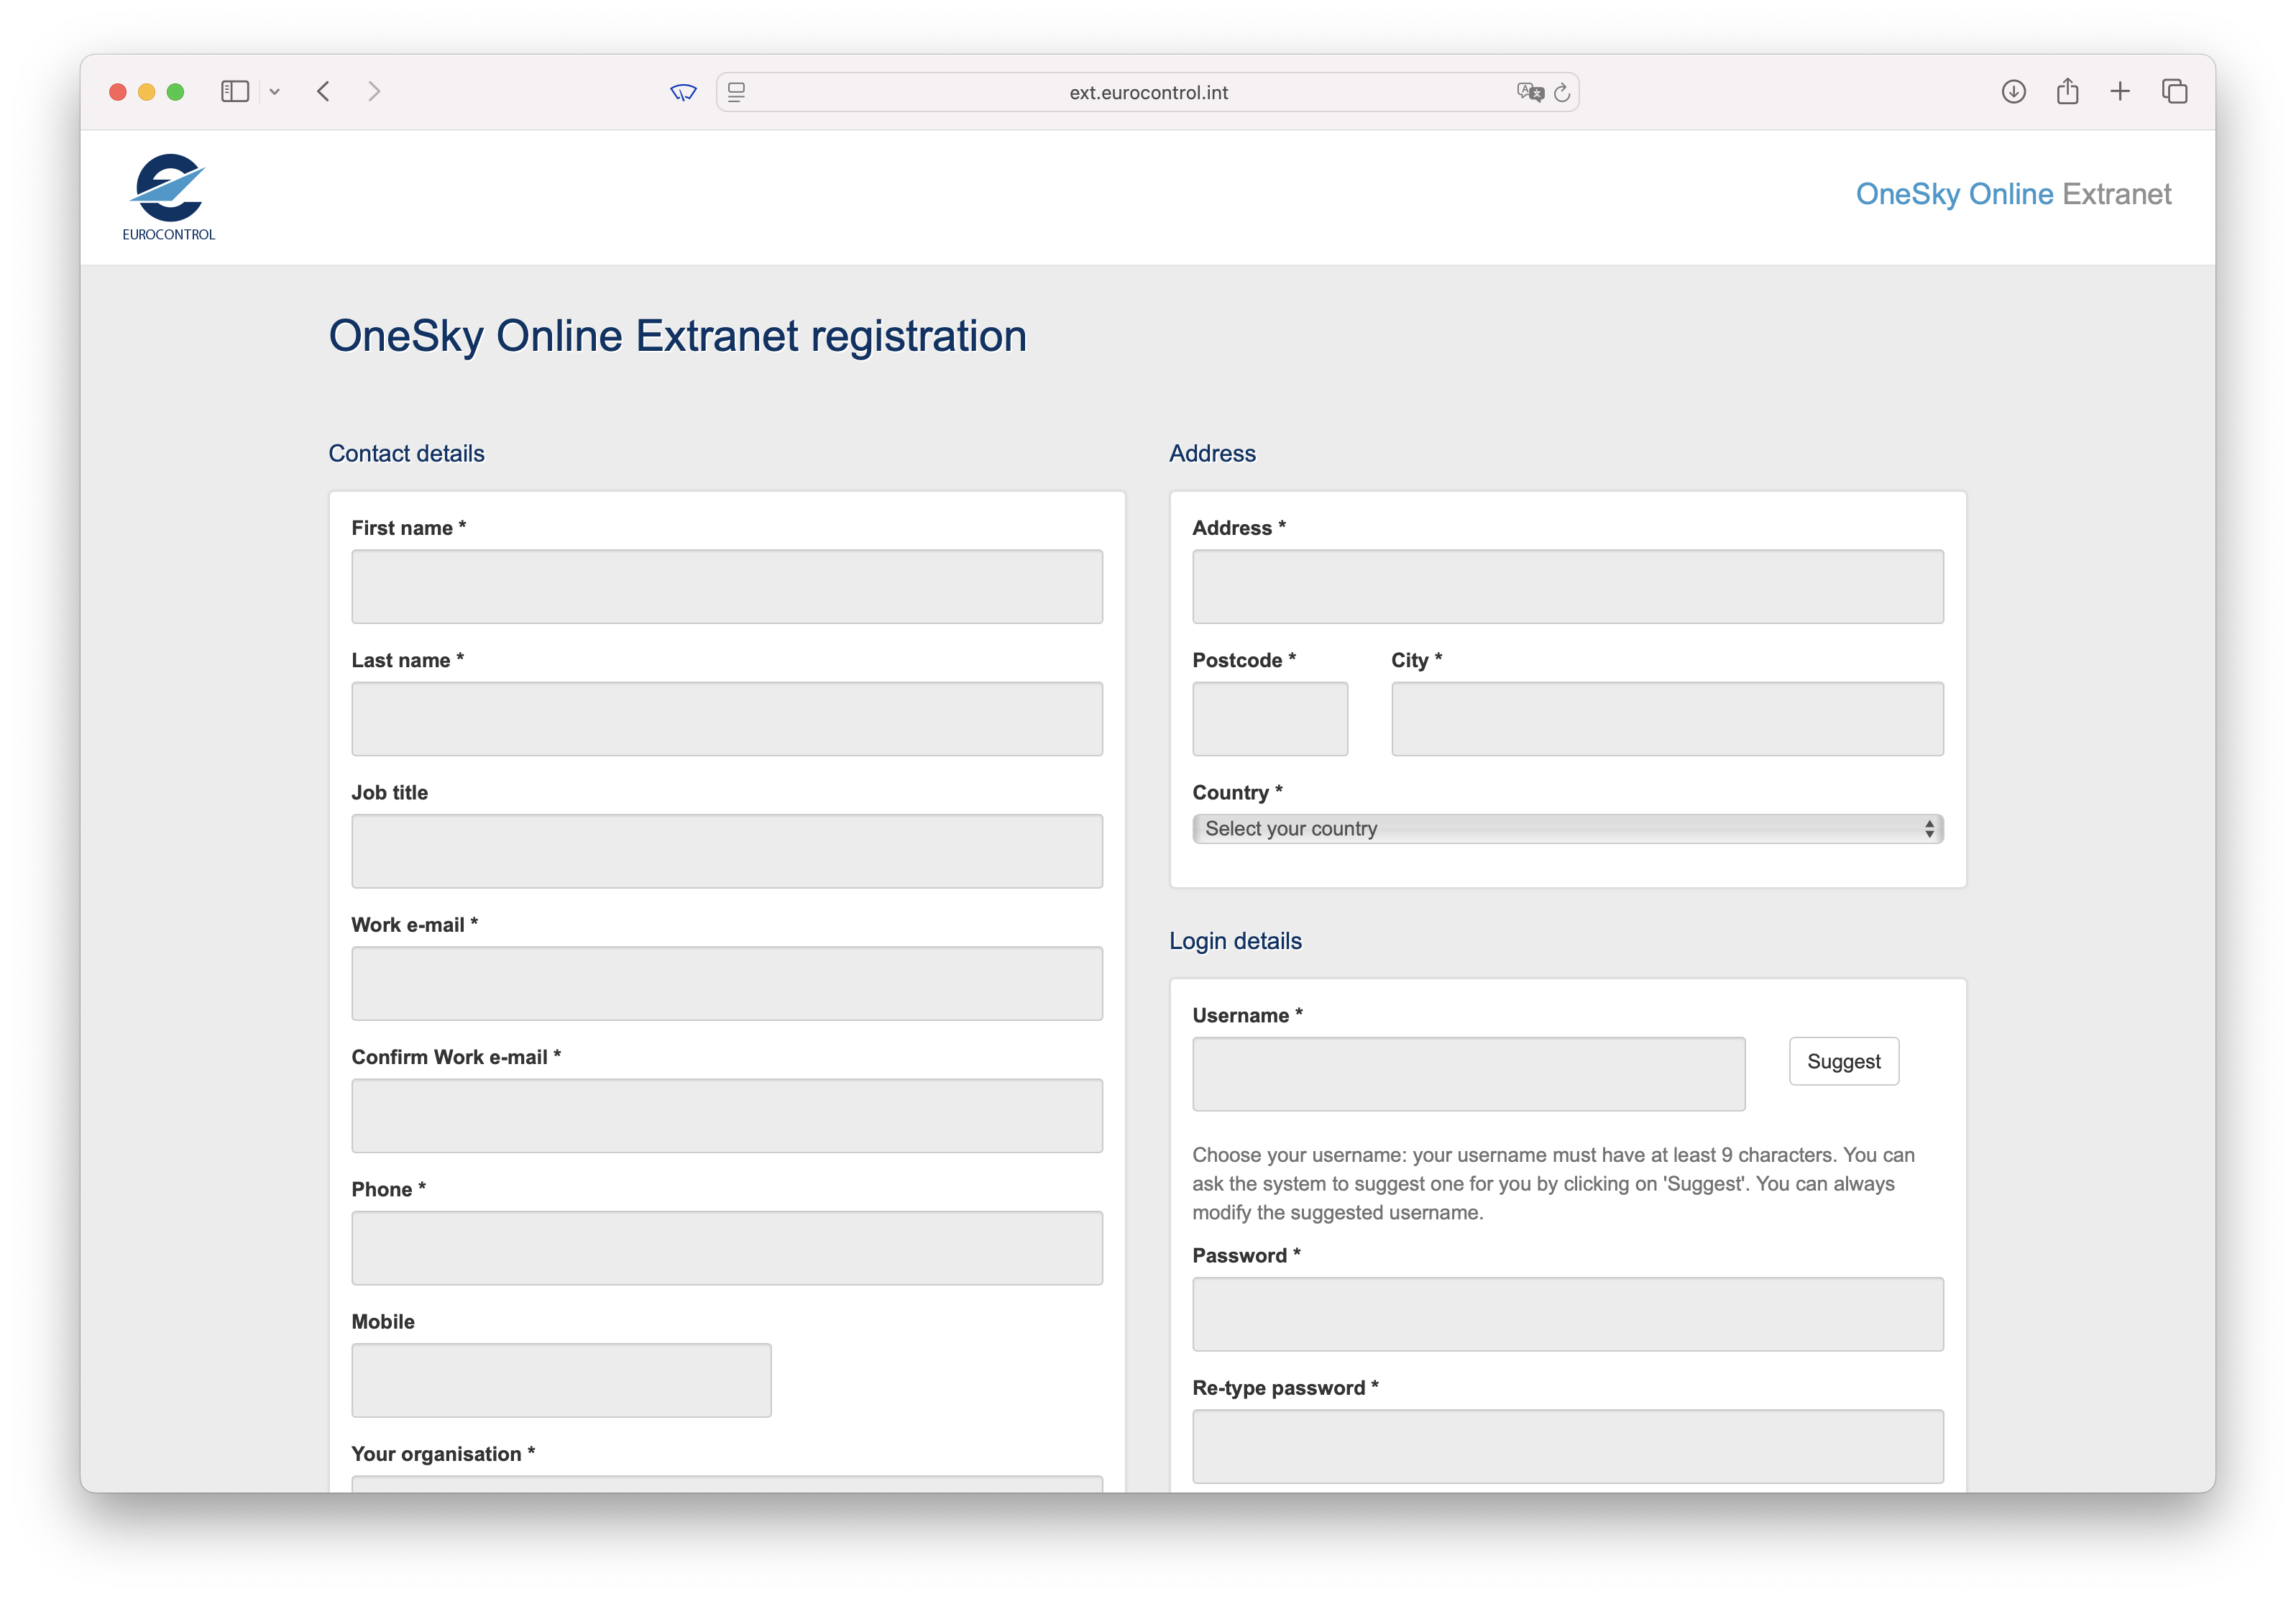
\includegraphics[width=\textwidth]{chapters/ch3/img/img-form.png}
    \subcaption{Registrazione sul OneSky Online~\cite{OneSky-account}.}
    \label{fig:account_creation}
  \end{subfigure}\hfill
  \begin{subfigure}[b]{0.5\textwidth}
    \centering
    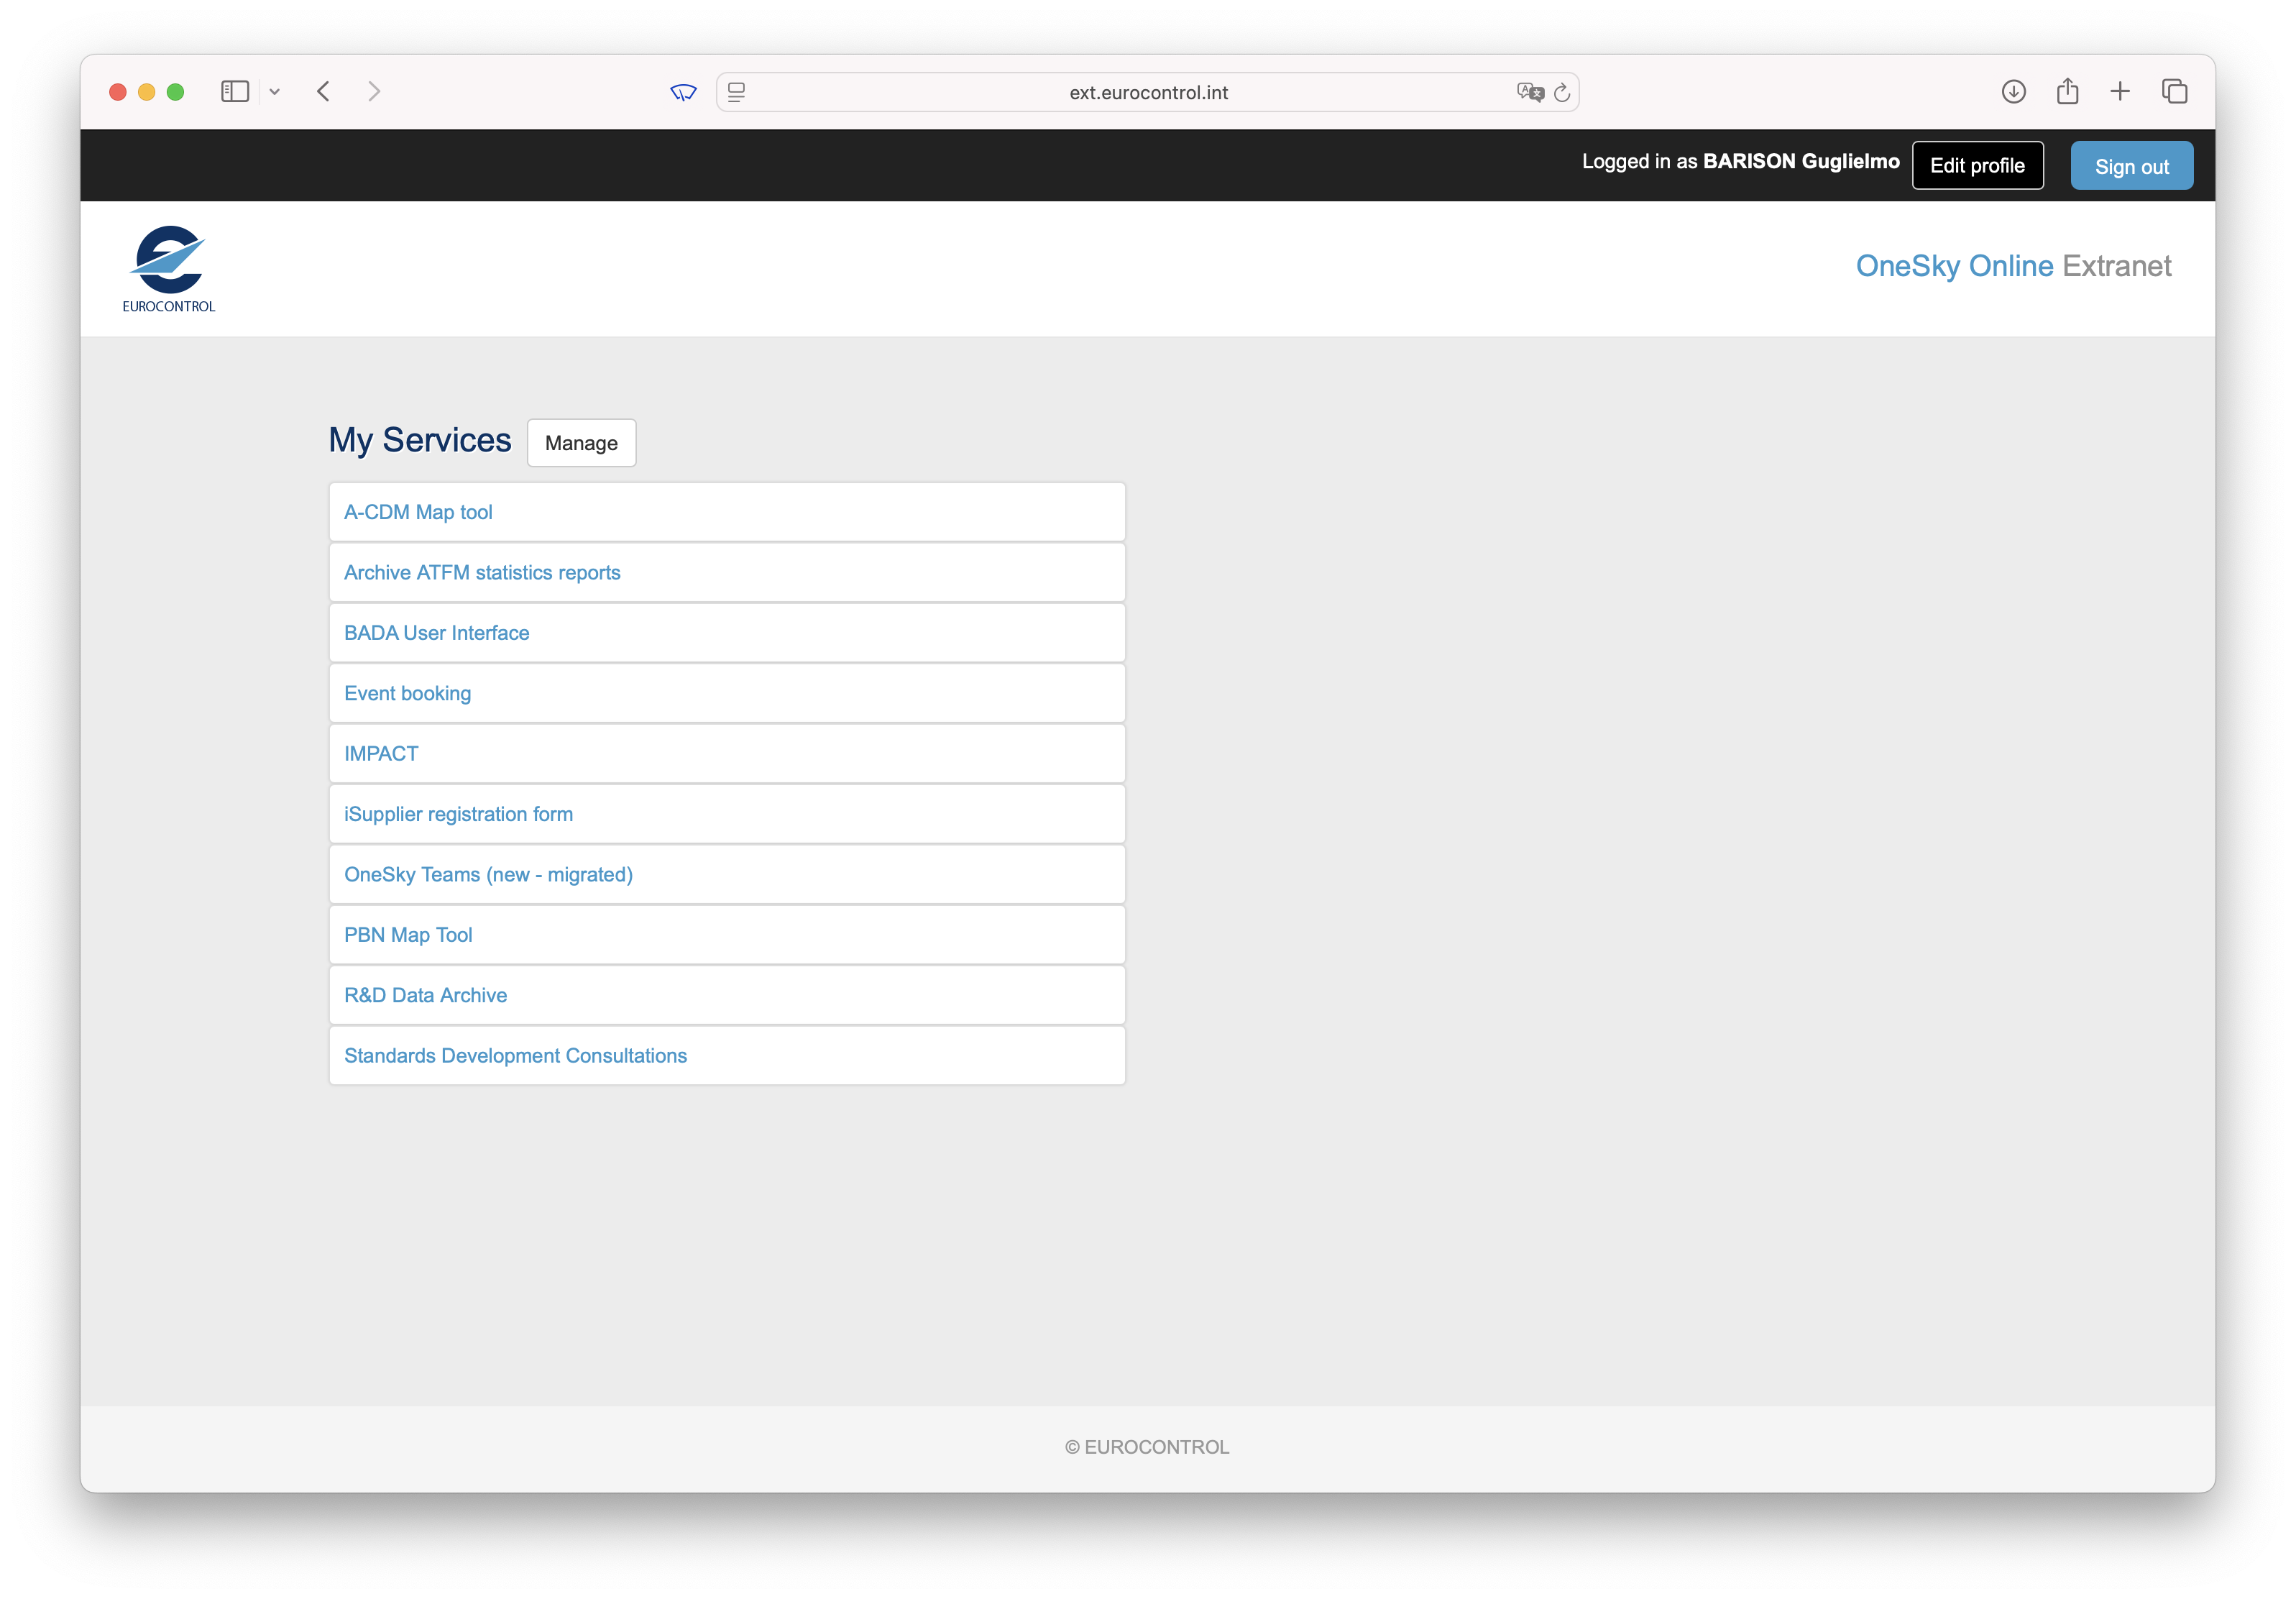
\includegraphics[width=\textwidth]{chapters/ch3/img/img-dashboard.png}
    \subcaption{Scelta del servizio ADRR~\cite{OneSky-adr}.}
    \label{fig:dataset_selection}
  \end{subfigure}
  % --- seconda coppia di immagini ---
  \begin{subfigure}[b]{0.5\textwidth}
    \centering
    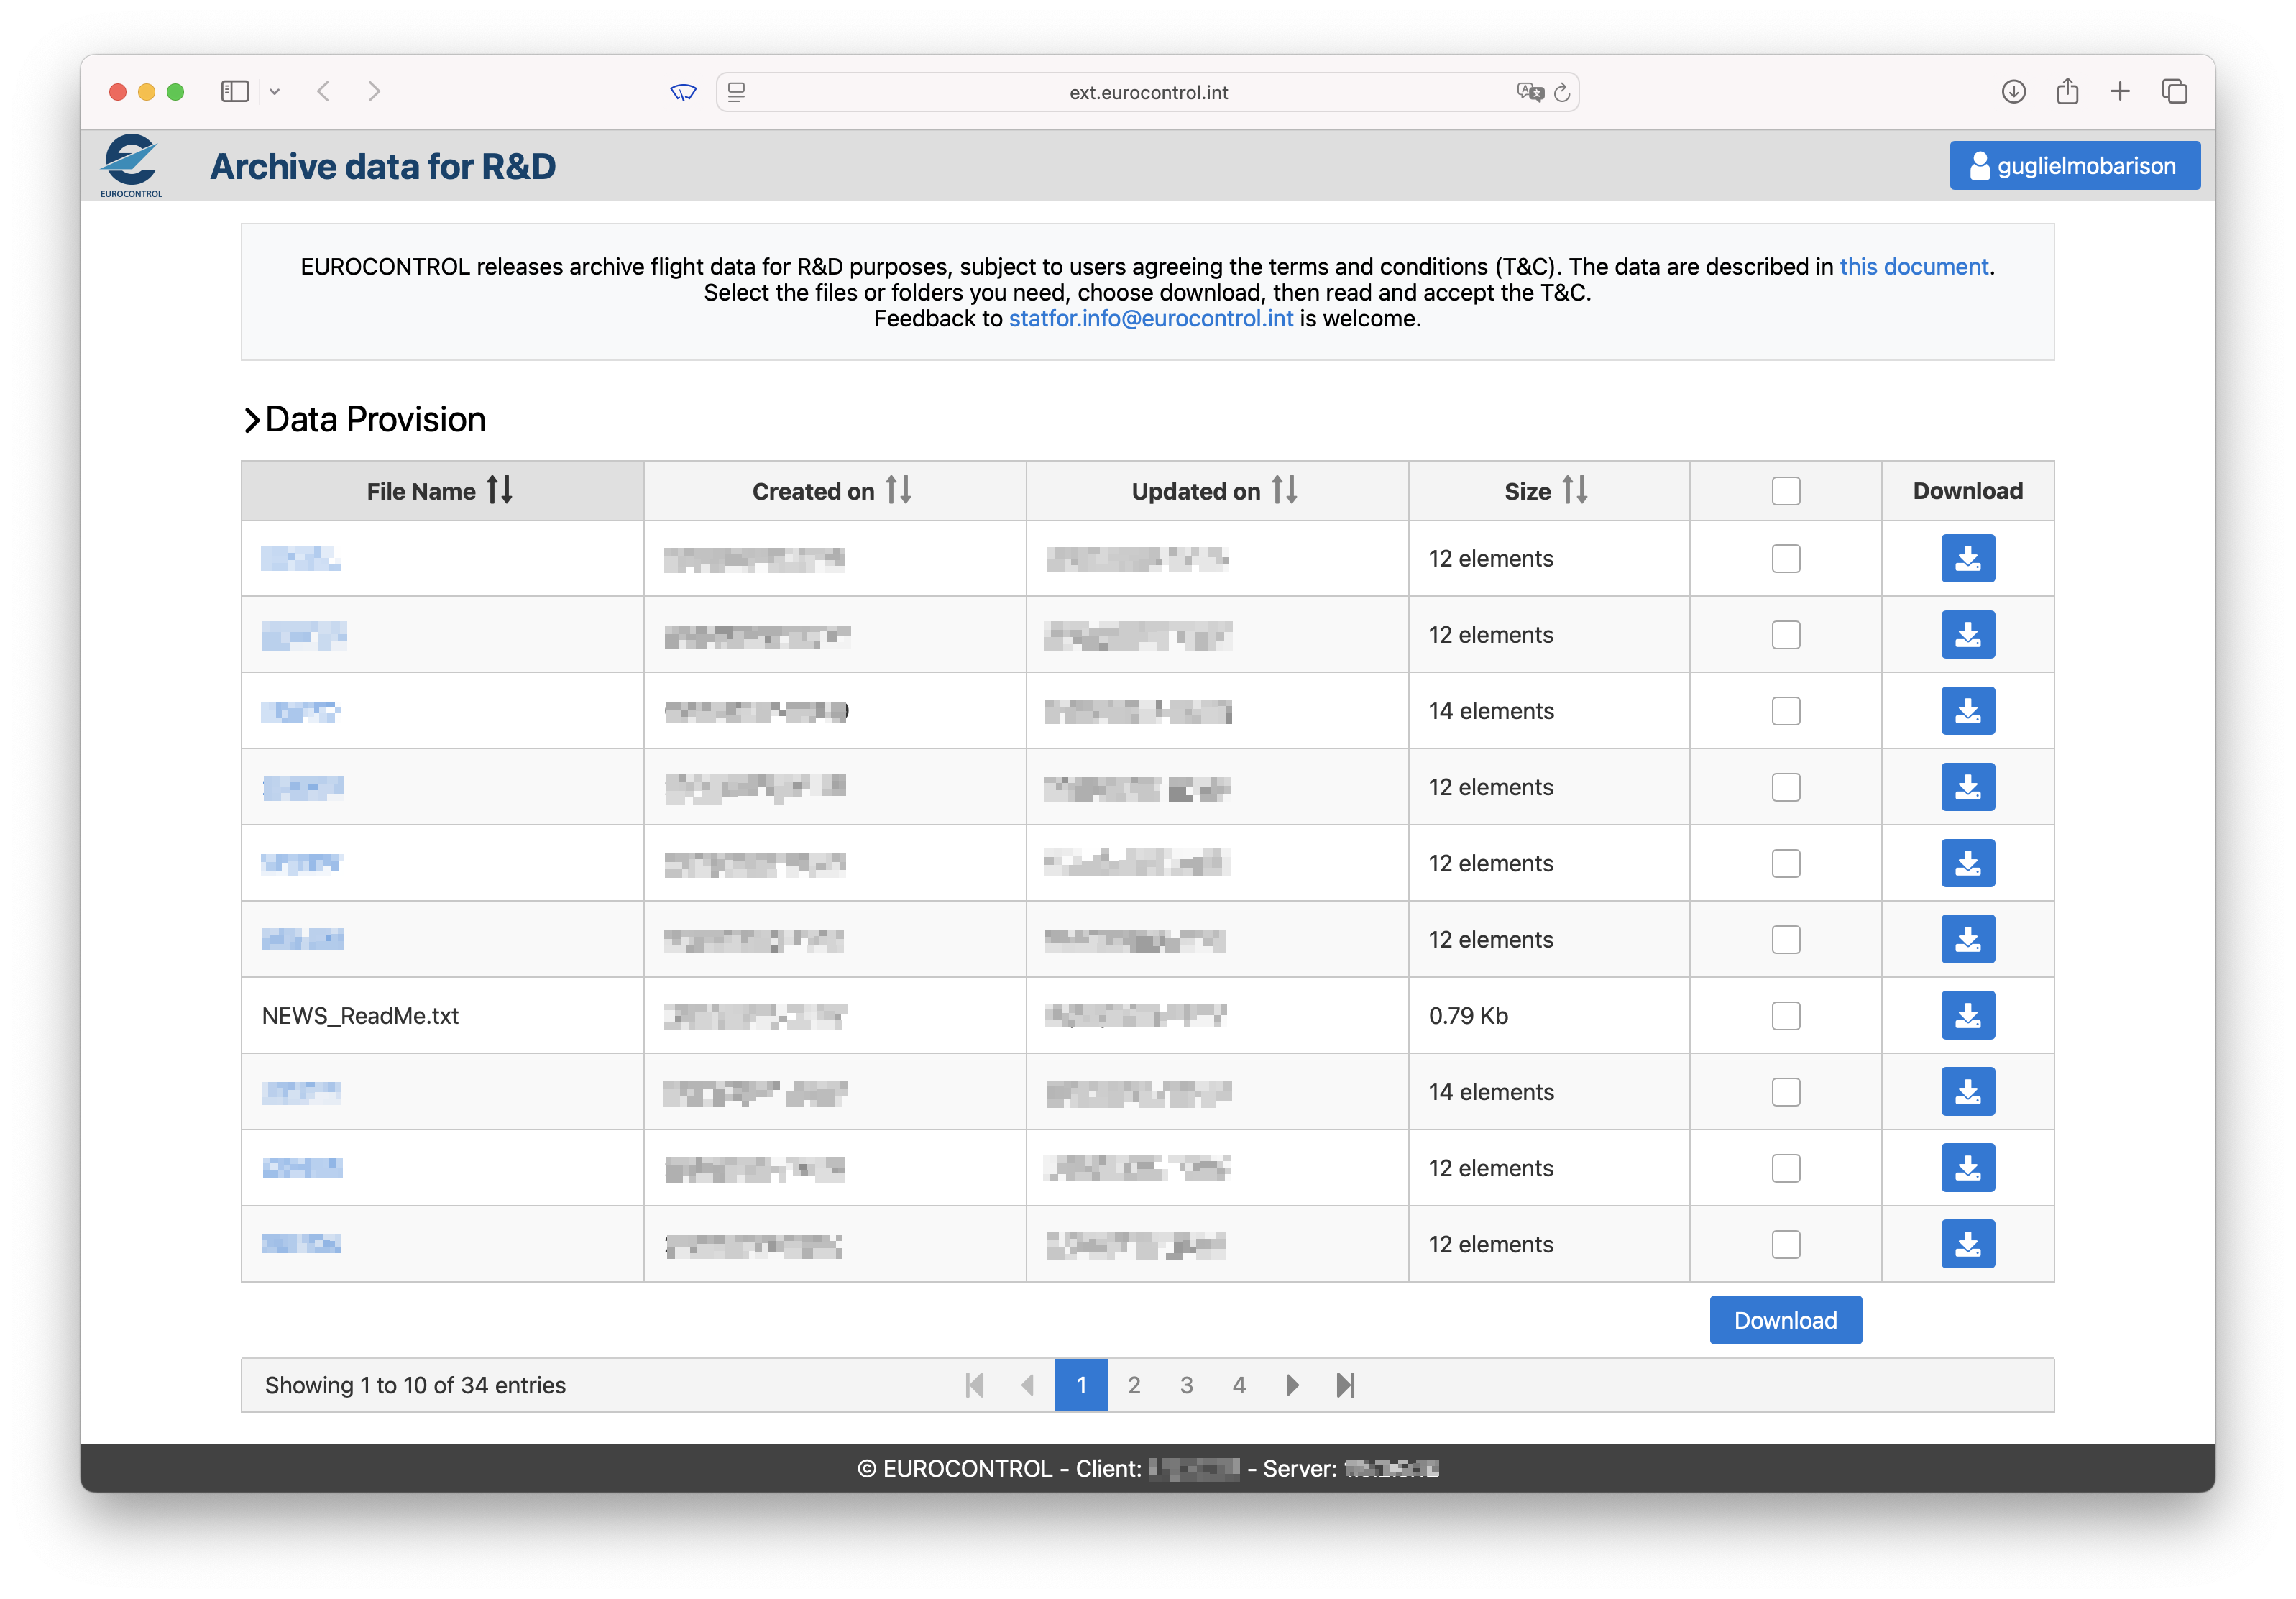
\includegraphics[width=\textwidth]{chapters/ch3/img/img-dashboard2.png}
    \subcaption{Scelta del dataset desiderato~\cite{OneSky-adr-dataset}.}
    \label{fig:terms_acceptance}
  \end{subfigure}\hfill
  \begin{subfigure}[b]{0.5\textwidth}
    \centering
    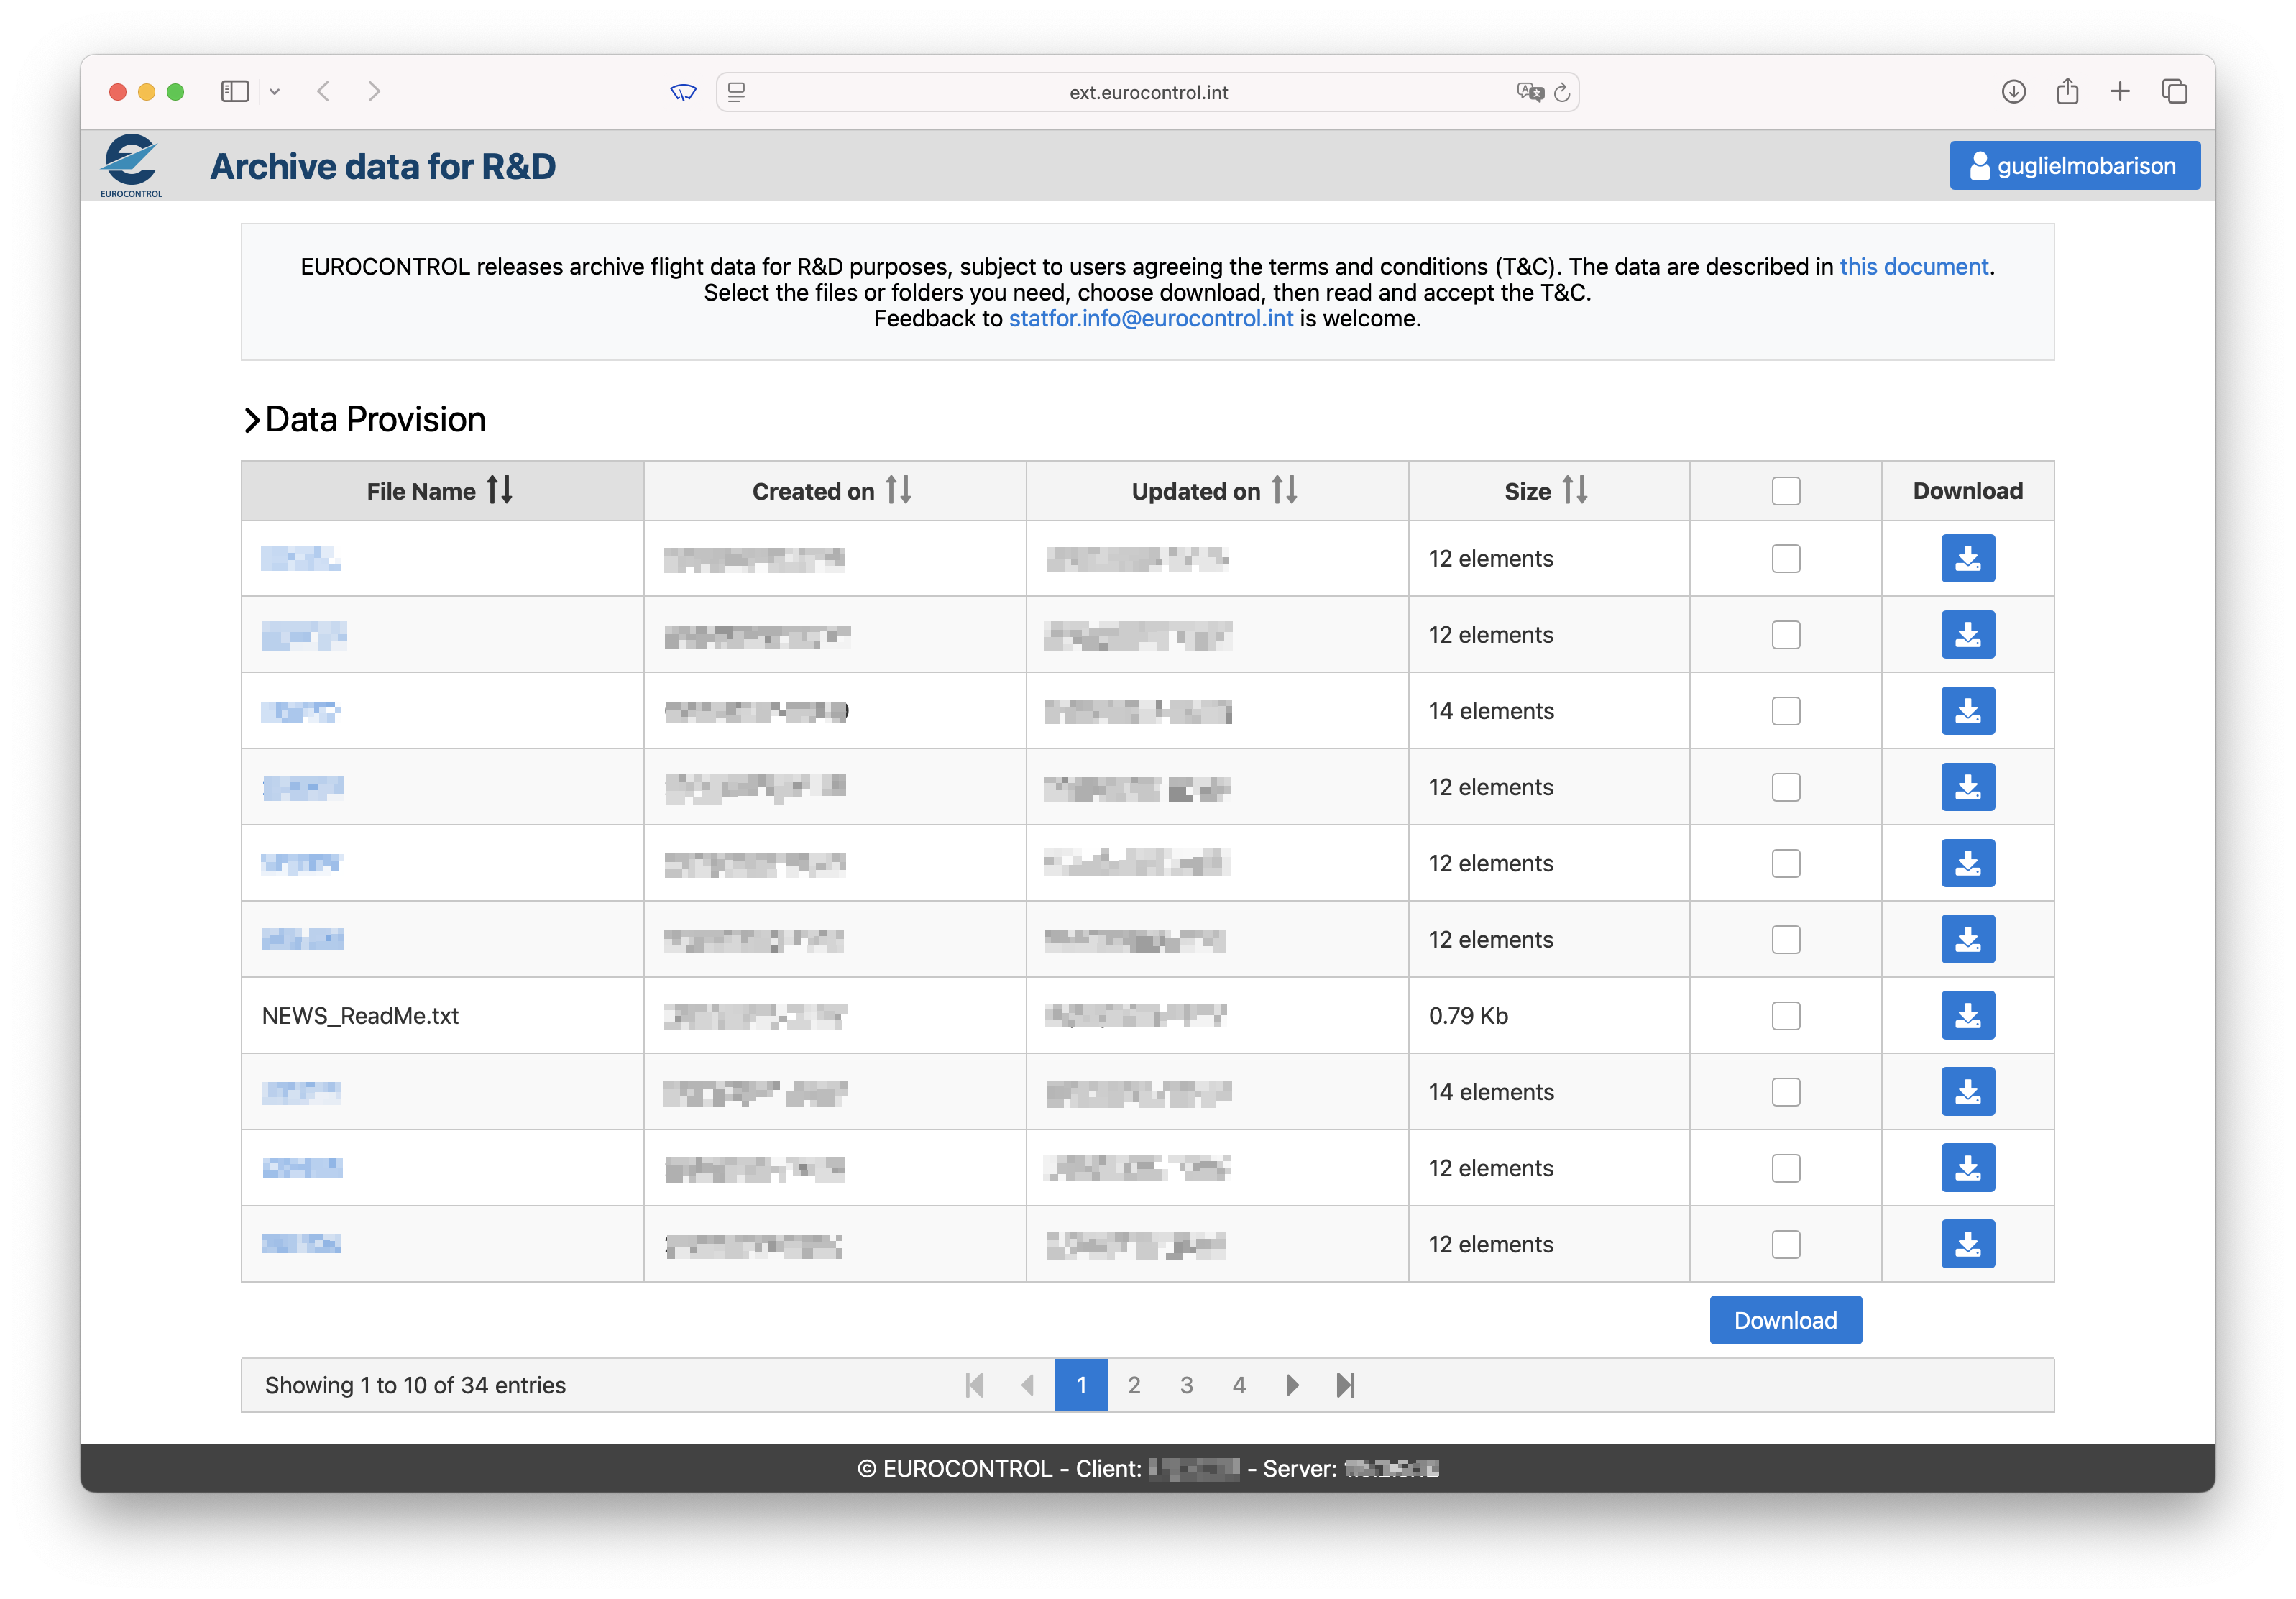
\includegraphics[width=\textwidth]{chapters/ch3/img/img-dashboard2.png}
    \subcaption{Dettaglio del dataset selezionato~\cite{OneSky-adr-dataset2}.}
    \label{fig:download_adrr}
  \end{subfigure}

  \caption{Procedure di accesso e condizioni d’uso del portale OneSky Online~\cite{eurocontrol2025onesky}.}
  \label{fig:accesso_conditions}
\end{figure}



\section{Origine e qualità dei dati}
I dataset \gls{adrr} derivano principalmente da due fonti principali:
\begin{description}
  \item[\gls{nm}:] Fornisce dati relativi ai piani di volo IFR e alle strutture dello spazio aereo.
  \item[\gls{crco}:] Contribuisce con aggiornamenti specifici riguardanti gli operatori e la registrazione degli aeromobili.
\end{description}
\clearpage
\subsection{Origine dei dati}
\DisablePunct
\begin{itemize}
\item \textbf{Dati di volo}
\begin{itemize}
\item \textbf{Dettagli dei voli (\textsection~\ref{sec:flights})}: provengono dai piani di volo \acrshort{ifr} depositati presso il \gls{nm}. Quando disponibili, le informazioni relative all'operatore e alla registrazione dell'aeromobile vengono integrate e corrette tramite aggiornamenti provenienti dal \gls{crco}.
\item \textbf{Profili di volo (\textsection\textsection~\ref{sec:flight_points} e~\ref{sec:flight_airspace})}: i profili \textit{filed} derivano direttamente dai piani di volo presentati al \gls{nm}, mentre i profili \textit{actual} sono ottenuti tramite osservazioni radar e messaggi \gls{atfcm} gestiti dal \gls{nm}.
\end{itemize}

\item \textbf{Dati ambientali (\textsection~\ref{sec:atm_env})}: estratti dal database di configurazione del \gls{nm}, comprendono strutture dello spazio aereo, rotte e cicli \gls{airac}, aggiornati regolarmente ad ogni ciclo operativo.
\end{itemize}
\EnablePunct\subsection{Qualità e validazione}
I dati sono forniti ``as‐is'' senza garanzie di qualità; eventuali correzioni sono basate sui meccanismi \gls{crco} e osservazioni radar, ma non viene garantita una validazione a posteriori completa.  
